\documentclass[aspectratio=169,12pt]{beamer}
%\documentclass[handout]{beamer}

% ### Preamble

% Encoding
\usepackage[utf8]{inputenc} % Use utf8 encoding in the input (.tex) file
\usepackage[english]{babel} % Load characters and hyphenation
\usepackage[T1]{fontenc} % Use utf8 encoding in the output (.pdf) file
\usepackage[english=british]{csquotes} % Quote like a boss

% Decorations
\usepackage{microtype} % Improves character and word spacing
\usepackage{booktabs} % Better horizontal rules in tables
\usepackage{multicol} % Customisation for tables
\usepackage{amsmath} % Improved mathematics

% Debug: grids
%\setbeamertemplate{background}[grid][step=1mm]

% Size
% With an aspect ratio of 16:9, I prefer having wide margins
\setbeamersize{text margin left=1.5cm}
\setbeamersize{text margin right=1.5cm}

% Presentation structure
\usepackage{appendixnumberbeamer} % Allows for an appendix

% Special content
\usepackage{textgreek} % Greek characters
\usepackage{units} % Used for printing standard units
\usepackage[scale=2]{ccicons} % Creative Commons icons

% Bibliography
\usepackage[sortcites,style=authoryear-icomp]{biblatex} % Bibliography
\addbibresource{../main.bib}
\AtEveryBibitem{
	\clearfield{url}
	\clearfield{issn}
	\clearfield{isbn}
	\clearfield{archivePrefix}
	\clearfield{arxivId}
	\clearfield{pmid}
	\clearfield{eprint}
	\clearfield{doi}
	\clearfield{number}
	\clearfield{pages}
	\clearfield{volume}
}

% Images
\usepackage{graphicx}
\usepackage{subcaption}
\graphicspath{ {../images/} }
\setkeys{Gin}{keepaspectratio} % Improves figure scaling
\setlength\abovecaptionskip{-5pt}
\setbeamerfont{caption}{size=\tiny} % Font size for captions

% Themes, colours and fonts
% Choose the theme according to the purpose of the presentation; do not 
% become too attached to a particular theme. For long presentations, a 
% sidebar which highlights the current topic can be helpful.
% Themes
\usetheme[
	progressbar=frametitle,
	%progressbar=foot,
	numbering=fraction,
	%sectionpage=simple,
	block=fill,
]{metropolis} % A modern theme
%\usetheme{Madrid} % A classic
%\usetheme{Hannover} % Side bar
% Colour themes
%\usecolortheme{seagull} % Gray-based
%\usecolortheme{crane} % Straw yellow
% Fonts
\usepackage{FiraSans} % Font needed by metropolis
\usepackage{FiraMono} % Font needed by metropolis
\usepackage{amsfonts} % Math fonts
\usepackage{xspace} % Print a space better than a ~

\newcommand{\etal}{\textit{et al.}\xspace}

%\definecolor{mLightBrown}{HTML}{EB811B}
%\newcommand{\alert}[1]{\textcolor{mLightBrown}{#1}} % Print text in 
%orange

% Table of contents
\setbeamertemplate{section in toc}[sections numbered] % ToC style
%\AtBeginSection[] % Recurring ToC
%{
%	\begin{frame}
%		\frametitle{Table of Contents}
%    	\tableofcontents[currentsection]
%	\end{frame}
%}

% Footer
% Remember: if everyone in the audience knows you, putting your name at 
% the bottom of each slide is just vanity.
%\setbeamertemplate{frame footer}{\tiny Footer} 

% Notes and printing layout settings

%

\usepackage{pgfpages} % Manage page layout 
%\pgfpagesuselayout{4 on 1}[a4paper,border shrink=0mm,landscape]
%\setbeameroption{show notes} % Print note after corresponding frame
%\setbeameroption{show only notes} % Print only notes
%\setbeameroption{show notes on second screen} % (Self explainatory)
%\setbeamertemplate{note page}[plain] % Use minimal notes

% ### Top matter

\title{Transcriptome-Wide Association Studies}
\subtitle{\footnotesize Bridging the gap between genome, transcriptome 
	and disease}
\author[Federico Marotta]
{
	\scriptsize
	Supervisor: \href{mailto:paolo.provero@unito.it}{Prof. Paolo 
		Provero}
	\\
	Candidate: \href{mailto:federico.marotta@edu.unito.it}{Federico 
		Marotta}
}
\institute[UniTo, DBMSS]
{
	\scriptsize
	\bigskip

	Università degli Studi di Torino\\
	Dipartimento di Biotecnologie Molecolari e Scienze per la Salute

	\bigskip
	\vfill

	{\tiny {\ccbysa\/}
	\href{https://creativecommons.org/licenses/by-sa/4.0/}
	{CC BY-SA}}
}
\date{\tiny Tesi di Laurea, 18 Luglio 2018}

% ### Document

\begin{document}

\maketitle

% Table of contents
% It can seem silly in a ten-minute presentation.
% NOTE: This frame is mutually exclusive with a recurring ToC.
%\begin{frame}
	%\frametitle{Outline}
	%\tableofcontents
%\end{frame}

\begin{frame}{Nature or Nurture: that is the question}

	\bigskip

	\begin{block}{Complex diseases:}
		As opposed to Mendelian diseases, complex ones cannot be 
explained by a mutation in a single gene
	\end{block}

	\bigskip

	Do they have a genetic basis at all?

	\pause

	\begin{itemize}
		\item Initially, there were \alert{linkage studies} and 
\alert{candidate-gene association studies}
		\item Gradually, the focus moved towards \alert{populations and 
whole genomes}
		\item \alert{GWAS}, especially if combined with eQTL mapping and 
functional annotations, have been useful
	 \end{itemize}

	\note[item]{Interaction of many genes with each other and with the 
environment}
	\note[item]{We have seen with Alessandro Lussana that non coding 
variants are important}
	\note[item]{To answer the question, many methods were developed}
	\note[item]{A linkage study is... a candidate-gene association study 
is... a GWAS is... eQTL mapping is...}
	\note[item]{Many SNP-disease association have been found}

\end{frame}

\begin{frame}{\ldots But GWAS do not explain everything}

	heritability

	mechanism

	interpretation and druggability

	GWAS: avere una A al posto di una C ti fa ammalare (non ha 
	significato).
	TWAS: se questo gene è più espresso, ci si ammala (molto più 
	interpretabile per un umano).

	\note[item]{Not only are they more difficult to interpret, but also 
to translate into clinical applications}

\end{frame}

\begin{frame}

	scheme of the pyramid

\end{frame}

\section{A gene-based association method \newline
\scriptsize Gamazon \etal (2015), \textit{Nature Genetics}}

% NOTE: excluding decomposition of gene expression, validation of 
% prediction (otherwise I should discuss heritability).

%\begin{frame}{Imputation of gene expression (?)}

	%\begin{columns}
		%\begin{column}{0.4\textwidth}
			%Since gene expression is not measured in a GWAS, it must be 
			%imputed
		%\end{column}

		%\begin{column}{0.6\textwidth}
			%\begin{figure}
				%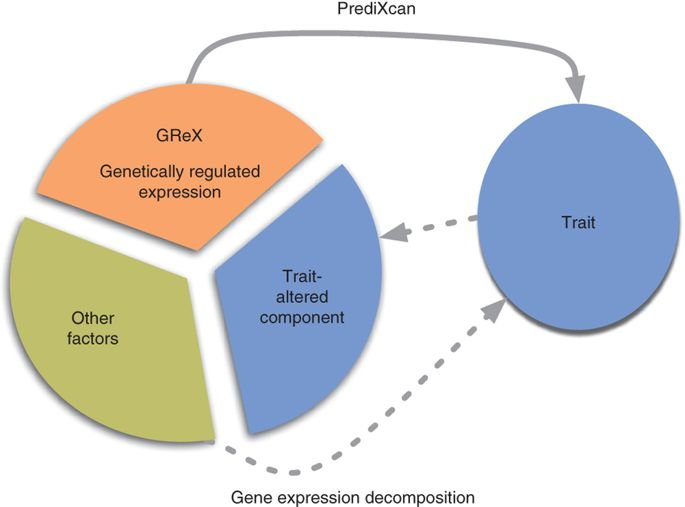
\includegraphics[width=\textwidth]{gamazon2015/1-expression_decomposition}
				%\caption{Expression can be decomposed in three 
				%components}
			%\end{figure}
		%\end{column}
	%\end{columns}

%\end{frame}

\begin{frame}{Training on reference transcriptome data sets}
	
	\begin{columns}
		\begin{column}{0.4\textwidth}
			Since gene expression is not measured in a GWAS, it must be 
imputed
		\end{column}

		\begin{column}{0.6\textwidth}
			\begin{figure}
				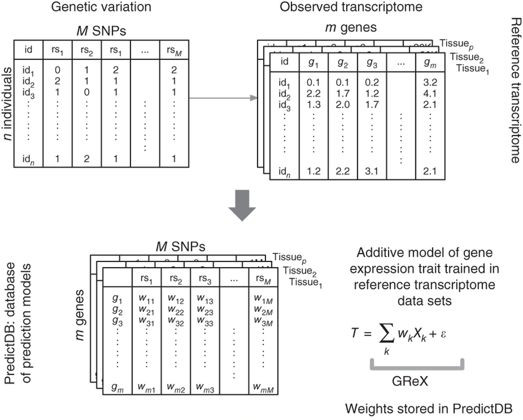
\includegraphics[width=\textwidth]{gamazon2015/2-grex_estimation_part1}
			\end{figure}
		\end{column}
	\end{columns}

	\note[item]{Phenotype-determined expression goes away because these 
are healthy individuals. The environment component goes away because it 
averages out in the regression model.}

\end{frame}

\begin{frame}{Association of the imputed expression to the phenotype}

	The expression predicted in each individual is then associated to 
its phenotype
	
	\begin{figure}
		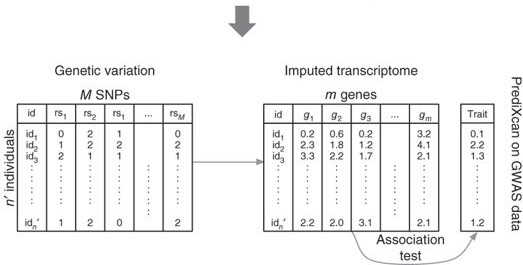
\includegraphics[width=0.8\textwidth]{gamazon2015/2-grex_estimation_part2}
	\end{figure}

	\note[item]{Logistic model. They could have modeled the liability to 
disease.}
	\note[item]{This is the real TWAS. The previous part was only needed 
because expression is not measured}

\end{frame}

\begin{frame}{Results}

	\begin{figure}
		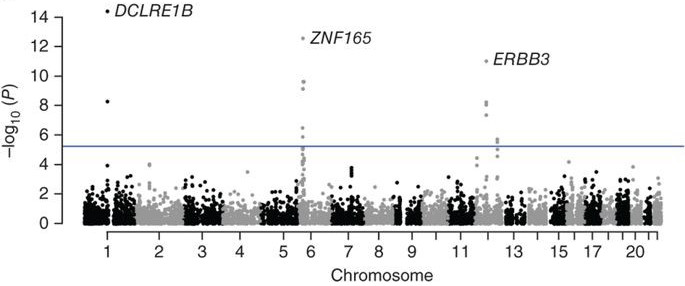
\includegraphics[width=0.8\textwidth]{gamazon2015/7-t1d_associations_manhattan}
	\end{figure}

	\note[item]{Why are nearby genes all associated? coregulation 
because of tad altered (upstream event)? This could be a pitfall of 
TWAS. See conclusions.}

\end{frame}

\section{Integrative approaches \newline
\scriptsize Gusev \etal (2016), \textit{Nature Genetics}}

\begin{frame}{From individual-level to summary-based TWAS}

	\begin{figure}
		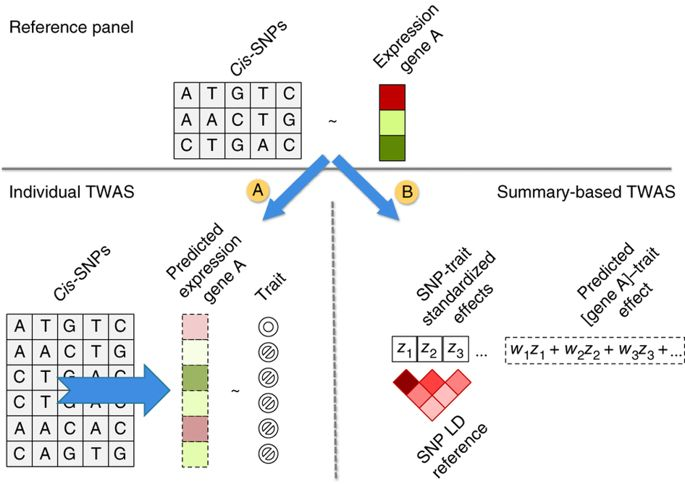
\includegraphics[width=0.8\textwidth]{gusev2016/1-TWAS_schematic}
	\end{figure}

	\note[item]{Individual-level data is not available}
	\note[item]{If a SNP is associated to a trait with score z_SNP, but 
it does not alter gene expression, its contribution to the association 
score of the gene to the trait is 0.}

\end{frame}

\begin{frame}{Application}

	The estimation of SNP weights was performed on \char`\~3000 
individuals

	\begin{itemize}
		\item When applied to a small-cohort GWAS, this approach found 
some genes that were reported in a later large-cohort GWAS
		\item 900,000 phenotypes
	\end{itemize}

	\note[item]{First bullet: TWAS are more powerful. Indeed, less 
multiple testing.}

\end{frame}

\section{Moving beyond genetic variants alone \newline
\scriptsize Gusev \etal (2018), \textit{Nature Genetics}}

% NOTE: here the results will be more important. Previously we have 
% neglected them.

\begin{frame}{Schematic}

	\begin{columns}
		\begin{column}{0.5\textwidth}
			\begin{figure}
				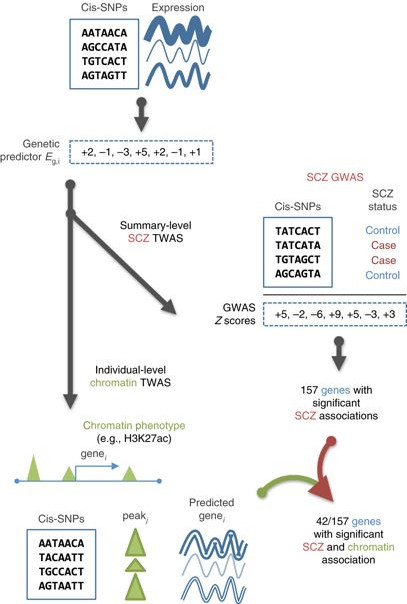
\includegraphics[width=\textwidth]{gusev2018/1-TWAS_schematic_cropped}
			\end{figure}
		\end{column}

		\begin{column}{0.5\textwidth}
			\begin{itemize}
				\item An association does not imply a causal mechanism
				\item Genetic variants
			\end{itemize}
		\end{column}
	\end{columns}

	\note[item]{Gene expression is one of the many intermediate 
phenotypes}

\end{frame}

\begin{frame}

	schizophrenia twas

	spliceome was

	chromatin twas

\end{frame}

\begin{frame}

	either mapk or klc1.

\end{frame}

\begin{frame}{Conclusions}

	additive models do not account for epistasis, dominance, penetrance

	more interpretability (anecdote of A->G vs. gene more or less 
expressed) and druggability

	not only expression: also structure

\end{frame}

\begin{frame}{Future perspectives}

	Association study-related:

	anything-WAS

	any population

	improvement of associations:

	take account of biological ideas (epistasis, dominance, penetrance)

	network to integrate and detect upstream events

\end{frame}

\appendix

\begin{frame}[allowframebreaks] % Allow citations to occupy many frames
	\frametitle{}
	\nocite{*}
	\tiny
	\printbibliography[title=References,keyword=TWAS]
\end{frame}

\begin{frame}{Different levels of phenotype}

	pyramid

\end{frame}

\begin{frame}{Comparison of TWAS with classical approaches}

	\begin{figure}
		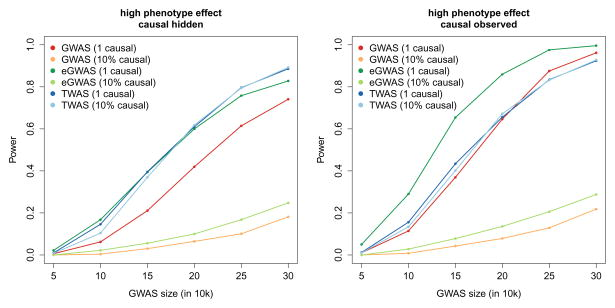
\includegraphics{gusev2016/5-association_power}
	\end{figure}

	\note[item]{Allelic heterogeneity}

\end{frame}

\end{document}

% ### Reference

% Dual screen with notes:

% To display notes on second screen, do the following. First you have to 
% set up the projector: open the display settings and choose "join 
% displays". (mirror just copies the pc monitor on the projector; single 
% display neglects one of the displays.) Set the built-in display as the 
% primary one. You can also set the resolution for each display, e.g. 
% for the PC you can set 16:9 and for the projector 4:3 or whatever is 
% available. This will create two displays, and you can switch from one 
% another moving the mouse cursor to the appropriate site.
% At this point you have to run the presentation, using a tool capable 
% to exploit dual screens. There are several options:
% pympress. On the command line, write pympress, then open the right 
% file. It does not always work, and the presentation in 16:9 does not 
% fit the projector display.
% dspdfviewer. On the command line, write dspdfviewer main.pdf. It will 
% work out of the box.
% pdfpc. On the command line, pdfpc main.pdf --notes=right. It can also 
% work out of the box, without the options. If you use the option 
% --notes, specify the same value you had specified to pgfpages inside 
% the .tex file. It also handles overlays (I still have to investigate 
% this feature). However, in dspdfviewer I can see both the current 
% slide and the notes; besides, the space for the notes is bigger.

% Graphics: figure environment

%\begin{figure}
%	\centering
%	\includegraphics[width=0.8\textwidth, keepaspectratio]{imgname}
%\end{figure}

% Interactive global structure: framezoom

%\framezoom<1><2>[border](5.5cm,0.5cm)(1cm,1cm)
%\begin{figure}
% 	\includegraphics[width=2cm,height=2cm]{imgname}
%\end{figure}
